\chapter{Penerapan Termodinamika Statistik}\label{ch:b3:statistical-thermo-applied}

Hidrogen cair yang disimpan dalam tangki berisolasi terbaik pun tetap
menguap, dan pada hari-hari pertama setelah pencairan penguapannya jauh lebih
cepat daripada yang dapat dijelaskan oleh kalor yang merembes melalui
dinding. Kalor itu berasal dari dalam cairan. Molekul hidrogen ada dalam dua
bentuk, yang hanya berbeda dalam orientasi relatif spin kedua protonnya dan
yang saling berubah satu menjadi yang lain dengan sangat lambat; pada
\qty{20}{K}, perubahan satu bentuk menjadi bentuk lainnya melepaskan kalor
yang lebih besar daripada yang diperlukan untuk menguapkan cairannya. Bab ini
menerapkan fungsi-fungsi partisi \cref{ch:b3:partition-functions} pada
kapasitas kalor, pada isomer-isomer spin inti ini, dan pada entropi yang
masih dimiliki sebagian kristal pada 0 K, lalu menghitung tetapan
kesetimbangan dan efek isotop dari data spektroskopi saja.

\begin{recall}
\Cref{ch:b3:partition-functions} menyusun \omterm{def:b3:partition-functions:partition-function}{fungsi partisi molekul} dan keempat
faktornya, serta menurunkan $U$, $S$ dan $G$ darinya. Jilid Tahun 2
mengaitkan tetapan kesetimbangan standar dengan energi Gibbs reaksi standar,
$\Delta_rG^\circ = -RT\ln K^\circ$, dan menetapkan persamaan van 't Hoff;
\cref{ch:b3:many-electron-atoms} menyatakan bahwa fungsi gelombang berganti
tanda ketika dua fermion identik dipertukarkan;
\cref{ch:b3:rovibrational-spectroscopy} mendapati selang-seling 3:1
intensitas garis dalam spektrum Raman rotasi molekul-molekul mirip \ce{H2}.
Bagian Kelas 9 dalam jilid pertama mendefinisikan isotop.
\end{recall}

\begin{omfigure}
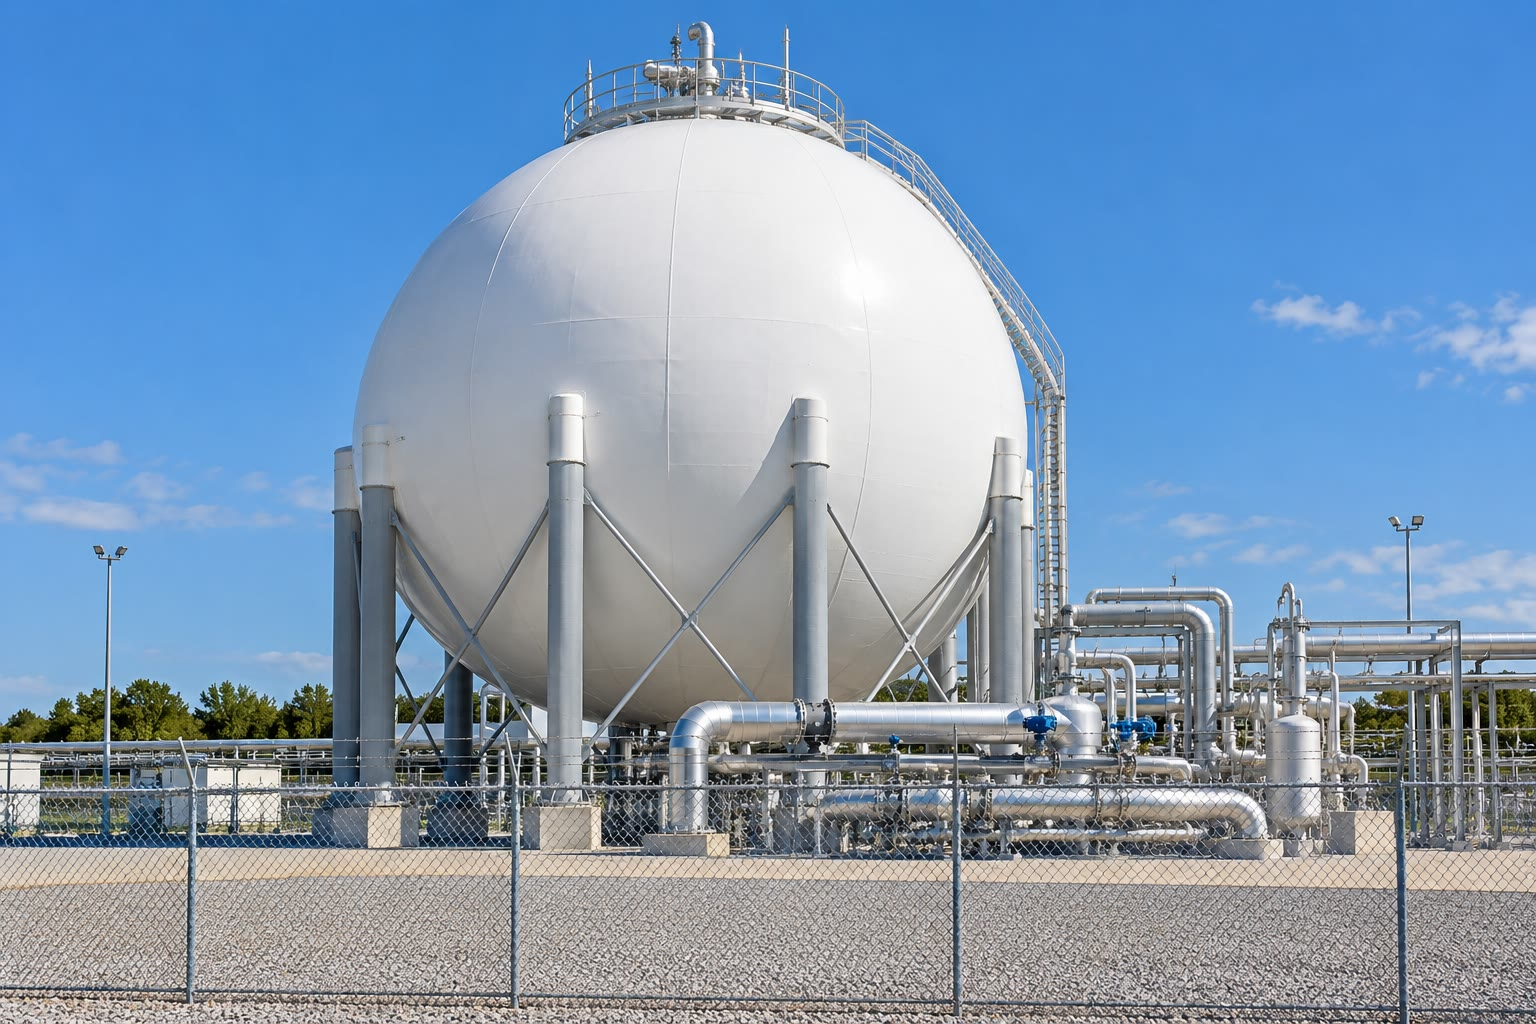
\includegraphics[width=0.6\linewidth]{images/book4/ai/b3-11-lh2-tank.jpg}

{\small Tangki bola untuk hidrogen cair. Pada \qty{20}{K}, kalor yang
dihasilkan di dalam cairan oleh perubahan lambat satu bentuk spin inti
hidrogen menjadi bentuk yang lain dapat melebihi kalor yang merembes masuk
dari luar.}
\end{omfigure}

\section{Kapasitas kalor gas}

Kapasitas kalor pada volume tetap adalah $C_V = (\partial U/\partial T)_V$, dan
menurut \cref{thm:b3:partition-functions:internal-energy} setiap jenis gerak
menyumbang secara terpisah. Dua limit menguasai segalanya.

\begin{theorem}[Teorema ekipartisi]\label{thm:b3:statistical-thermo-applied:equipartition}
Jika tingkat-tingkat energi sebuah gerak rapat dibandingkan dengan $kT$,
setiap suku energinya yang kuadratik dalam sebuah koordinat atau sebuah
momentum menyumbang $\frac12kT$ pada energi rata-rata sebuah molekul, sehingga
$\frac12R$ pada kapasitas kalor molar. Pernyataan ini disebut \emph{teorema
ekipartisi}\index{teorema ekipartisi}.
\end{theorem}

\begin{proof}[Bukti parsial]
Dalam limit klasik, jumlah atas keadaan-keadaan sebuah gerak menjadi integral,
dan suku kuadratik $a u^2$ menyumbang faktor $\int\eu^{-\beta au^2}\dd u =
\sqrt{\pi/\beta a}$, yang sebanding dengan $\beta^{-1/2}$. Menurut
\cref{thm:b3:partition-functions:internal-energy}, energi rata-ratanya adalah
$-\partial\ln(\beta^{-1/2})/\partial\beta = 1/2\beta = \frac12kT$. Bahwa integral klasik
adalah limit jumlah kuantum telah ditunjukkan untuk translasi dan rotasi dalam
\cref{ch:b3:partition-functions}; untuk vibrasi, hal itu mengikuti proposisi
berikut jika $T \gg \theta_{\mathrm V}$.
\end{proof}

Translasi mempunyai tiga suku kuadratik ($\frac32R$); rotasi molekul linear
dua ($R$), rotasi molekul nonlinear tiga ($\frac32R$); setiap vibrasi dua, kinetik
dan potensial ($R$). Jadi molekul linear dengan $N$ atom menuju
$C_{V,\mathrm m} = \frac52R + (3N - 5)R$ pada suhu tinggi. Limit itu hampir tidak
pernah tercapai untuk vibrasi pada suhu kamar.

\begin{proposition}[Kapasitas kalor vibrasi]\label{prop:b3:statistical-thermo-applied:cv-vib}
Vibrasi harmonik dengan suhu karakteristik $\theta_{\mathrm V}$ menyumbang, dengan
$x = \theta_{\mathrm V}/T$,
\[
  \frac{C_{V,\mathrm m}^{\mathrm V}}{R} = \frac{x^2\eu^x}{(\eu^x - 1)^2},
\]
yaitu fungsi Einstein, yang menuju 1 jika $T \gg \theta_{\mathrm V}$ dan turun secara
eksponensial, seperti $x^2\eu^{-x}$, jika $T \ll \theta_{\mathrm V}$.
\end{proposition}

\begin{proof}
Dari \cref{prop:b3:partition-functions:q-vib}, $U - U(0) = R\theta_{\mathrm V}/(\eu^x - 1)$ per
mol. Menurunkannya terhadap $T$, dengan $\dd x/\dd T = -x/T$, memberikan
$R\theta_{\mathrm V}\eu^x(x/T)/(\eu^x - 1)^2 = Rx^2\eu^x/(\eu^x - 1)^2$. Untuk $x \to 0$,
$\eu^x - 1 \approx x$ dan rasionya menuju 1; untuk $x$ yang besar, rasio itu
berperilaku seperti $x^2\eu^{-x}$.
\end{proof}

\begin{method}[Kapasitas kalor gas dari modus-modusnya]\label{met:b3:statistical-thermo-applied:cv}
\begin{enumerate}
  \item Translasi: $\frac32R$, selalu.
  \item Rotasi: $R$ (linear) atau $\frac32R$ (nonlinear) jika $T \gg \theta_{\mathrm R}$,
        yang berlaku untuk setiap gas kecuali hidrogen di atas beberapa puluh
        kelvin.
  \item Vibrasi: satu suku Einstein untuk setiap \omterm{def:b3:group-theory-applied:normal-mode}{modus normal}, dengan
        $\theta_{\mathrm V} = hc\tilde\nu/k$ dari bilangan gelombang fundamentalnya;
        modus terdegenerasi dihitung sebanyak \omterm{def:b3:quantum-model-systems:degenerate}{degenerasinya}.
  \item Jumlahkan, dan $C_{p,\mathrm m} = C_{V,\mathrm m} + R$ untuk gas ideal.
\end{enumerate}
\end{method}

Sebuah gerak dikatakan membeku jika $kT$ kecil dibandingkan dengan eksitasi
pertamanya: gerak itu lalu tidak menyimpan energi dan tidak menyumbang apa
pun pada $C_V$. Vibrasi \ce{N2} ($\theta_{\mathrm V} = \qty{3352}{K}$) membeku pada suhu
kamar dan $C_{V,\mathrm m} = \frac52R$; vibrasi \ce{Cl2} ($\theta_{\mathrm V} = \qty{798}{K}$)
setengah terjaga, $C_{V,\mathrm m} = 3.07R$ pada \qty{300}{K}.

\begin{omfigure}
\begin{tikzpicture}
\begin{axis}[width=0.86\linewidth, height=6.4cm, xmode=log, xmin=10, xmax=3000,
  ymin=1.3, ymax=3.9, axis lines=left, xlabel={$T$ / K}, ylabel={$C_{V,\mathrm m}/R$},
  tick label style={font=\small}, label style={font=\small},
  log ticks with fixed point, xtick={10,30,100,300,1000,3000},
  unbounded coords=jump]
\addplot[omDef, thick] table[x=T, y=N2] {figdata/out/bachelor-3-heat-capacity.dat};
\addplot[black!60, thick] table[x=T, y=Cl2] {figdata/out/bachelor-3-heat-capacity.dat};
\addplot[omThm, thick, dashed] table[x=T, y=nH2] {figdata/out/bachelor-3-heat-capacity.dat};
\addplot[omThm, thick] table[x=T, y=eH2] {figdata/out/bachelor-3-heat-capacity.dat};
\addplot[only marks, mark=*, mark size=1.6pt, omDef] table[x=T, y=N2] {figdata/out/bachelor-3-heat-capacity-janaf.dat};
\addplot[only marks, mark=square*, mark size=1.5pt, black!60] table[x=T, y=Cl2] {figdata/out/bachelor-3-heat-capacity-janaf.dat};
\draw[black!30, densely dotted] (axis cs:10,1.5) -- (axis cs:3000,1.5);
\draw[black!30, densely dotted] (axis cs:10,2.5) -- (axis cs:3000,2.5);
\draw[black!30, densely dotted] (axis cs:10,3.5) -- (axis cs:3000,3.5);
\node[font=\scriptsize, black!60, anchor=south east] at (axis cs:2900,1.5) {$\frac32$: translasi};
\node[font=\scriptsize, black!60, anchor=south west] at (axis cs:10.5,2.5) {$\frac52$: + rotasi};
\node[font=\scriptsize, black!60, anchor=south west] at (axis cs:10.5,3.5) {$\frac72$: + vibrasi};
\node[font=\scriptsize, omThm, anchor=south west] at (axis cs:60,3.6) {\ce{H2} kesetimbangan};
\node[font=\scriptsize, omThm, anchor=north west] at (axis cs:130,1.78) {\ce{H2} normal};
\node[font=\scriptsize, black!70, anchor=south east] at (axis cs:560,3.33) {\ce{Cl2}};
\node[font=\scriptsize, omDef, anchor=south east] at (axis cs:1000,3.0) {\ce{N2}};
\end{axis}
\end{tikzpicture}

{\small Kapasitas kalor molar pada volume tetap, yang dihitung dari
tetapan-tetapan spektroskopi (garis; \omterm{def:b3:quantum-model-systems:rotor}{rotor tegar}, vibrasi harmonik), bersama
nilai-nilai tabel termokimia untuk \ce{N2} dan \ce{Cl2} (titik, $C_p/R - 1$).
Vibrasi mulai terjaga di sekitar $\theta_{\mathrm V}/10$; di atas sekitar
\qty{1000}{K} nilai tabel naik di atas model harmonik, yang mengabaikan
anharmonisitas. Hidrogen: sumbangan rotasi hidrogen normal (garis putus-putus,
orto dan para membeku pada 3:1) dan hidrogen kesetimbangan (garis penuh), yang
melampaui $\frac52$ karena perubahan para menjadi orto menyerap kalor.}
\end{omfigure}

\section{Statistik spin inti}

Kedua inti \ce{H2} adalah fermion identik. Mempertukarkannya mengubah tanda
fungsi gelombang total (\cref{ch:b3:many-electron-atoms}); mempertukarkannya
sama dengan membalik molekul ujung ke ujung, yang mengalikan fungsi gelombang
rotasi $Y_{J,M}$ dengan $(-1)^J$ dan fungsi spin inti dengan $+1$ atau $-1$.

\begin{theorem}[Statistik spin inti]\label{thm:b3:statistical-thermo-applied:spin-statistics}
Dalam molekul diatomik homonuklir yang intinya berspin $I$, dengan keadaan
elektronik dasar ${}^1\Sigma_g^+$, terdapat $(2I+1)(I+1)$ keadaan spin inti yang
simetris dan $(2I+1)I$ yang antisimetris. Untuk fermion ($I$ setengah bulat),
keadaan-keadaan antisimetris menyertai $J$ genap dan yang simetris menyertai
$J$ ganjil; untuk boson ($I$ bulat) sebaliknya. Untuk \ce{H2} ($I = \frac12$),
tingkat genap dan ganjil mempunyai bobot spin 1 dan 3; untuk \ce{D2} ($I = 1$),
6 dan 3. Jika $I = 0$, hanya satu paritas $J$ yang ada sama sekali: molekul
\ce{CO2} yang linear, dengan dua inti \ce{^{16}O} dan keadaan dasar yang
simetris, hanya mempunyai tingkat-tingkat rotasi genap.
\end{theorem}

\begin{proof}[Bukti parsial]
Postulat simetri (fungsi gelombang total antisimetris terhadap pertukaran dua
fermion identik, simetris untuk boson) diterima tanpa bukti. Ke-$(2I+1)^2$ hasil
kali keadaan spin satu inti $|m_1\rangle|m_2\rangle$ memberikan $2I+1$ keadaan
simetris dengan $m_1 = m_2$, dan untuk setiap pasangan dari $(2I+1)2I/2$
pasangan $m_1 \ne m_2$, satu kombinasi simetris dan satu antisimetris:
$(2I+1) + (2I+1)I = (2I+1)(I+1)$ keadaan simetris dan $(2I+1)I$ keadaan
antisimetris. Dalam keadaan ${}^1\Sigma_g^+$, fungsi elektronik dan fungsi
vibrasinya tidak berubah oleh pertukaran itu, sehingga hasil kali fungsi
rotasi dan fungsi spin harus mempunyai tanda keseluruhan yang disyaratkan:
untuk fermion, $(-1)^J \times(\text{simetri spin}) = -1$, yang memasangkan
$J$ genap dengan keadaan-keadaan spin antisimetris. Untuk \ce{H2}: 3 simetris,
1 antisimetris; untuk \ce{D2}: 6 dan
3.
\end{proof}

\begin{definition}[Hidrogen orto dan para]\label{def:b3:statistical-thermo-applied:spin-isomers}
Yang disebut \emph{hidrogen orto}\index{hidrogen orto} adalah bentuk \ce{H2}
yang kedua spin protonnya berada dalam keadaan simetris (triplet), yang hanya
menempati tingkat-tingkat rotasi ganjil; yang disebut \emph{hidrogen
para}\index{hidrogen para} adalah bentuk dengan keadaan spin antisimetris
(singlet), yang hanya menempati tingkat-tingkat genap.
\end{definition}

Mengubah bentuk yang satu menjadi bentuk yang lain memerlukan pembalikan
satu spin inti relatif terhadap yang lain, sesuatu yang hampir tidak dapat
dilakukan oleh tumbukan dengan molekul hidrogen lain: dalam hidrogen murni
kedua bentuk itu berperilaku selama berhari-hari sebagai dua gas yang berbeda.
Permukaan paramagnetik, yang medan magnetnya tak homogen dan bekerja secara
berbeda pada kedua proton, mengatalisis perubahan itu.

\begin{proposition}[Rasio orto--para pada kesetimbangan]\label{prop:b3:statistical-thermo-applied:ortho-para}
Pada kesetimbangan, fraksi \omterm{def:b3:statistical-thermo-applied:spin-isomers}{hidrogen para} adalah
\[
  x_{\mathrm{para}} = \frac{\sum_{J\,\mathrm{even}}(2J+1)\eu^{-\theta_{\mathrm R}J(J+1)/T}}
    {\sum_{J\,\mathrm{even}}(2J+1)\eu^{-\theta_{\mathrm R}J(J+1)/T} + 3\sum_{J\,\mathrm{odd}}(2J+1)\eu^{-\theta_{\mathrm R}J(J+1)/T}},
\]
yang menuju 1 pada 0 K dan menuju $\frac14$ pada suhu tinggi. Untuk \ce{D2},
bentuk orto ($J$ genap) menuju 1 pada 0 K dan menuju $\frac23$ pada suhu tinggi.
\end{proposition}

\begin{proof}
\omterm{def:b3:partition-functions:boltzmann}{Distribusi Boltzmann} atas semua keadaan, dengan bobot spin dari
\cref{thm:b3:statistical-thermo-applied:spin-statistics}. Pada 0 K hanya $J = 0$,
yang genap, terpopulasi. Pada suhu tinggi, jumlah genap dan jumlah ganjil
masing-masing setengah dari $T/\theta_{\mathrm R}$, dan rasionya $1 : 3$; untuk \ce{D2},
$6 : 3$.
\end{proof}

Untuk \ce{H2}, $\theta_{\mathrm R} = \qty{85.4}{K}$: campuran kesetimbangannya setengah
para pada \qty{78}{K}, 99.8\,\% para pada titik didihnya, \qty{20.37}{K}, dan
25.07\,\% pada suhu kamar. Hidrogen yang disimpan pada suhu kamar, yang
disebut hidrogen normal, karena itu merupakan campuran orto dan para 3:1.

\begin{omfigure}
\begin{tikzpicture}
\begin{axis}[width=0.72\linewidth, height=5.4cm, xmin=0, xmax=300, ymin=0, ymax=1.05,
  axis lines=left, xlabel={$T$ / K}, ylabel={fraksi kesetimbangan},
  tick label style={font=\small}, label style={font=\small}]
\addplot[omThm, thick] table[x=T, y=pH2] {figdata/out/bachelor-3-ortho-para.dat};
\addplot[omDef, thick] table[x=T, y=oD2] {figdata/out/bachelor-3-ortho-para.dat};
\draw[black!35, densely dotted] (axis cs:0,0.25) -- (axis cs:300,0.25);
\draw[black!35, densely dotted] (axis cs:0,0.6667) -- (axis cs:300,0.6667);
\node[font=\scriptsize, omThm, anchor=south west] at (axis cs:190,0.27) {fraksi para \ce{H2} $\to \frac14$};
\node[font=\scriptsize, omDef, anchor=south west] at (axis cs:120,0.69) {fraksi orto \ce{D2} $\to \frac23$};
\end{axis}
\end{tikzpicture}

{\small Komposisi kesetimbangan isomer-isomer spin inti terhadap suhu, dari
tingkat-tingkat rotasi dan bobot spinnya (\ce{H2}: 1 dan 3; \ce{D2}: 6 dan 3).
Kedua bentuk dengan $J$ genap mendominasi pada suhu rendah.}
\end{omfigure}

Kapasitas kalor hidrogen memperlihatkan akibat-akibatnya. Dalam hidrogen
normal, molekul orto dan para adalah dua gas yang tercampur dalam proporsi
tetap; masing-masing mempunyai tangga tingkatnya sendiri, mulai dari $J = 1$
dan dari $J = 0$, dan rotasinya membeku secara terpisah. Dalam hidrogen
kesetimbangan, pemanasan juga mengubah para menjadi orto, yang menyerap energi
dan menghasilkan puncak pada gambar di atas. Pengukuran-pengukuran pertama,
yang dilakukan tanpa katalis, mengikuti kurva hidrogen normal, dan tafsiran
kurva itu sebagai campuran 3:1 yang membeku itulah yang pertama kali
mengungkap kedua bentuk tersebut.

\begin{remark}
\omterm{def:b3:partition-functions:symmetry-number}{Bilangan simetri} dalam \cref{prop:b3:partition-functions:q-rot} kini dapat
dibenarkan. Pada suhu tinggi, setiap keadaan spin mendapati sekitar setengah
tingkat rotasi yang diizinkan, sehingga
$\sum(\text{bobot spin})(2J+1)\eu^{\dots} \approx (2I+1)^2\,T/2\theta_{\mathrm R}$: faktor
spin total $(2I+1)^2$ ditinggalkan menurut konvensi, dan tersisa $\sigma = 2$.
\end{remark}

\begin{definition}[Entropi sisa]\label{def:b3:statistical-thermo-applied:residual-entropy}
Yang disebut \emph{entropi sisa}\index{entropi sisa} sebuah kristal adalah
entropi yang masih dimilikinya ketika $T \to 0$ karena molekul-molekulnya
tetap membeku dalam salah satu dari banyak susunan yang energinya sama atau
hampir sama.
\end{definition}

\begin{proposition}[Entropi sisa karbon monoksida dan es]\label{prop:b3:statistical-thermo-applied:residual}
Kristal $N$ molekul yang membeku dalam $W_0$ susunan yang sama peluangnya
mempunyai $S_0 =
k\ln W_0$. \ce{CO} padat, yang setiap molekulnya dapat mengarah ke salah satu
dari dua arah, mempunyai $S_{0,\mathrm m} = R\ln2 =
\qty{5.76}{J.K^{-1}.mol^{-1}}$. Es, yang setiap oksigennya terikat pada dua atom
hidrogen dan berikatan hidrogen dengan dua atom lain, mempunyai
$W_0 = (3/2)^N$ dan $S_{0,\mathrm m} = R\ln\frac32 =
\qty{3.37}{J.K^{-1}.mol^{-1}}$.
\end{proposition}

\begin{proof}
\cref{def:b3:partition-functions:statistical-entropy} diterapkan pada $T \to 0$.
\ce{CO}: dipol molekulnya begitu kecil sehingga orientasi CO dan OC hampir
sama energinya, dan setiap molekul dari $N$ molekul mempunyai dua orientasi:
$W_0 = 2^N$, $S_0 = Nk\ln2$. Es (hitungan Pauling): setiap atom hidrogen dari
$2N$ atom hidrogen terletak pada sebuah garis O$\cdots$O, di dekat salah satu
ujungnya: $2^{2N}$ susunan. Dari 16 cara menempatkan keempat hidrogen di
sekitar satu oksigen, 6 cara memberinya tepat dua hidrogen dekat (sebuah
molekul air); dengan memperlakukan oksigen-oksigen itu sebagai saling bebas,
fraksi $6/16$ dari susunan-susunan itu memenuhi syarat untuk setiap oksigen:
$W_0 = 2^{2N}(6/16)^N = (3/2)^N$.
\end{proof}

Untuk \ce{CO}, tabel-tabel mengutip \omterm{def:b3:partition-functions:statistical-entropy}{entropi statistiknya}
(\cref{ch:b3:partition-functions}); nilai kalorimetrinya lebih rendah dengan
selisih yang berorde $R\ln2$, sedikit lebih kecil karena orientasinya tidak
sepenuhnya acak. Untuk es, selisih antara entropi kalorimetri uap air dan nilai
statistiknya sesuai dengan hitungan Pauling ketika ia membuatnya pada tahun
1935, yang mengukuhkan bahwa proton-proton dalam es tidak teratur. Hukum
ketiga, dalam bentuk ``entropi kristal sempurna adalah nol pada 0 K'', berlaku
untuk kristal-kristal yang memang mencapai satu susunan tunggal.

\begin{omfigure}
\begin{tikzpicture}[scale=1.15, every node/.style={transform shape}]
  \draw[black!45, dashed] (0.00,0.00) -- (1.20,0.00);
  \draw[black, thick] (0.00,0.00) -- (0.36,0.00); \node[aH, minimum size=2.2mm] at (0.36,0.00) {};
  \draw[black!45, dashed] (0.00,0.00) -- (0.00,1.20);
  \draw[black, thick] (0.00,0.00) -- (0.00,0.36); \node[aH, minimum size=2.2mm] at (0.00,0.36) {};
  \draw[black!45, dashed] (0.00,1.20) -- (1.20,1.20);
  \draw[black, thick] (0.00,1.20) -- (0.36,1.20); \node[aH, minimum size=2.2mm] at (0.36,1.20) {};
  \draw[black!45, dashed] (0.00,1.20) -- (0.00,2.40);
  \draw[black, thick] (0.00,2.40) -- (0.00,2.04); \node[aH, minimum size=2.2mm] at (0.00,2.04) {};
  \draw[black!45, dashed] (0.00,2.40) -- (1.20,2.40);
  \draw[black, thick] (1.20,2.40) -- (0.84,2.40); \node[aH, minimum size=2.2mm] at (0.84,2.40) {};
  \draw[black!45, dashed] (0.00,2.40) -- (0.00,3.60);
  \draw[black, thick] (0.00,3.60) -- (0.00,3.24); \node[aH, minimum size=2.2mm] at (0.00,3.24) {};
  \draw[black!45, dashed] (0.00,3.60) -- (1.20,3.60);
  \draw[black, thick] (1.20,3.60) -- (0.84,3.60); \node[aH, minimum size=2.2mm] at (0.84,3.60) {};
  \draw[black!45, dashed] (0.00,3.60) -- (0.00,4.20);
  \draw[black, thick] (0.00,3.60) -- (0.00,3.96); \node[aH, minimum size=2.2mm] at (0.00,3.96) {};
  \draw[black!45, dashed] (1.20,0.00) -- (2.40,0.00);
  \draw[black, thick] (1.20,0.00) -- (1.56,0.00); \node[aH, minimum size=2.2mm] at (1.56,0.00) {};
  \draw[black!45, dashed] (1.20,0.00) -- (1.20,1.20);
  \draw[black, thick] (1.20,1.20) -- (1.20,0.84); \node[aH, minimum size=2.2mm] at (1.20,0.84) {};
  \draw[black!45, dashed] (1.20,1.20) -- (2.40,1.20);
  \draw[black, thick] (2.40,1.20) -- (2.04,1.20); \node[aH, minimum size=2.2mm] at (2.04,1.20) {};
  \draw[black!45, dashed] (1.20,1.20) -- (1.20,2.40);
  \draw[black, thick] (1.20,1.20) -- (1.20,1.56); \node[aH, minimum size=2.2mm] at (1.20,1.56) {};
  \draw[black!45, dashed] (1.20,2.40) -- (2.40,2.40);
  \draw[black, thick] (1.20,2.40) -- (1.56,2.40); \node[aH, minimum size=2.2mm] at (1.56,2.40) {};
  \draw[black!45, dashed] (1.20,2.40) -- (1.20,3.60);
  \draw[black, thick] (1.20,3.60) -- (1.20,3.24); \node[aH, minimum size=2.2mm] at (1.20,3.24) {};
  \draw[black!45, dashed] (1.20,3.60) -- (2.40,3.60);
  \draw[black, thick] (2.40,3.60) -- (2.04,3.60); \node[aH, minimum size=2.2mm] at (2.04,3.60) {};
  \draw[black!45, dashed] (1.20,3.60) -- (1.20,4.20);
  \draw[black!45, dashed] (2.40,0.00) -- (3.60,0.00);
  \draw[black, thick] (3.60,0.00) -- (3.24,0.00); \node[aH, minimum size=2.2mm] at (3.24,0.00) {};
  \draw[black!45, dashed] (2.40,0.00) -- (2.40,1.20);
  \draw[black, thick] (2.40,0.00) -- (2.40,0.36); \node[aH, minimum size=2.2mm] at (2.40,0.36) {};
  \draw[black!45, dashed] (2.40,1.20) -- (3.60,1.20);
  \draw[black, thick] (2.40,1.20) -- (2.76,1.20); \node[aH, minimum size=2.2mm] at (2.76,1.20) {};
  \draw[black!45, dashed] (2.40,1.20) -- (2.40,2.40);
  \draw[black, thick] (2.40,2.40) -- (2.40,2.04); \node[aH, minimum size=2.2mm] at (2.40,2.04) {};
  \draw[black!45, dashed] (2.40,2.40) -- (3.60,2.40);
  \draw[black, thick] (3.60,2.40) -- (3.24,2.40); \node[aH, minimum size=2.2mm] at (3.24,2.40) {};
  \draw[black!45, dashed] (2.40,2.40) -- (2.40,3.60);
  \draw[black, thick] (2.40,2.40) -- (2.40,2.76); \node[aH, minimum size=2.2mm] at (2.40,2.76) {};
  \draw[black!45, dashed] (2.40,3.60) -- (3.60,3.60);
  \draw[black, thick] (2.40,3.60) -- (2.76,3.60); \node[aH, minimum size=2.2mm] at (2.76,3.60) {};
  \draw[black!45, dashed] (2.40,3.60) -- (2.40,4.20);
  \draw[black!45, dashed] (3.60,0.00) -- (4.20,0.00);
  \draw[black, thick] (3.60,0.00) -- (3.96,0.00); \node[aH, minimum size=2.2mm] at (3.96,0.00) {};
  \draw[black!45, dashed] (3.60,0.00) -- (3.60,1.20);
  \draw[black, thick] (3.60,1.20) -- (3.60,0.84); \node[aH, minimum size=2.2mm] at (3.60,0.84) {};
  \draw[black!45, dashed] (3.60,1.20) -- (4.20,1.20);
  \draw[black!45, dashed] (3.60,1.20) -- (3.60,2.40);
  \draw[black, thick] (3.60,1.20) -- (3.60,1.56); \node[aH, minimum size=2.2mm] at (3.60,1.56) {};
  \draw[black!45, dashed] (3.60,2.40) -- (4.20,2.40);
  \draw[black!45, dashed] (3.60,2.40) -- (3.60,3.60);
  \draw[black, thick] (3.60,2.40) -- (3.60,2.76); \node[aH, minimum size=2.2mm] at (3.60,2.76) {};
  \draw[black!45, dashed] (3.60,3.60) -- (4.20,3.60);
  \draw[black, thick] (3.60,3.60) -- (3.96,3.60); \node[aH, minimum size=2.2mm] at (3.96,3.60) {};
  \draw[black!45, dashed] (3.60,3.60) -- (3.60,4.20);
  \draw[black, thick] (3.60,3.60) -- (3.60,3.96); \node[aH, minimum size=2.2mm] at (3.60,3.96) {};
  \draw[black!45, dashed] (-0.60,0.00) -- (0.00,0.00);
  \draw[black!45, dashed] (-0.60,1.20) -- (0.00,1.20);
  \draw[black, thick] (0.00,1.20) -- (-0.36,1.20); \node[aH, minimum size=2.2mm] at (-0.36,1.20) {};
  \draw[black!45, dashed] (-0.60,2.40) -- (0.00,2.40);
  \draw[black, thick] (0.00,2.40) -- (-0.36,2.40); \node[aH, minimum size=2.2mm] at (-0.36,2.40) {};
  \draw[black!45, dashed] (-0.60,3.60) -- (0.00,3.60);
  \draw[black!45, dashed] (0.00,-0.60) -- (0.00,0.00);
  \draw[black!45, dashed] (1.20,-0.60) -- (1.20,0.00);
  \draw[black, thick] (1.20,0.00) -- (1.20,-0.36); \node[aH, minimum size=2.2mm] at (1.20,-0.36) {};
  \draw[black!45, dashed] (2.40,-0.60) -- (2.40,0.00);
  \draw[black, thick] (2.40,0.00) -- (2.40,-0.36); \node[aH, minimum size=2.2mm] at (2.40,-0.36) {};
  \draw[black!45, dashed] (3.60,-0.60) -- (3.60,0.00);
  \node[aO, minimum size=4mm] at (0.00,0.00) {};
  \node[aO, minimum size=4mm] at (0.00,1.20) {};
  \node[aO, minimum size=4mm] at (0.00,2.40) {};
  \node[aO, minimum size=4mm] at (0.00,3.60) {};
  \node[aO, minimum size=4mm] at (1.20,0.00) {};
  \node[aO, minimum size=4mm] at (1.20,1.20) {};
  \node[aO, minimum size=4mm] at (1.20,2.40) {};
  \node[aO, minimum size=4mm] at (1.20,3.60) {};
  \node[aO, minimum size=4mm] at (2.40,0.00) {};
  \node[aO, minimum size=4mm] at (2.40,1.20) {};
  \node[aO, minimum size=4mm] at (2.40,2.40) {};
  \node[aO, minimum size=4mm] at (2.40,3.60) {};
  \node[aO, minimum size=4mm] at (3.60,0.00) {};
  \node[aO, minimum size=4mm] at (3.60,1.20) {};
  \node[aO, minimum size=4mm] at (3.60,2.40) {};
  \node[aO, minimum size=4mm] at (3.60,3.60) {};
\end{tikzpicture}

{\small Ketakteraturan proton dalam es, digambar sebagai jaringan persegi datar
(jaringan sebenarnya tetrahedral): setiap oksigen (merah) mempunyai empat
tetangga O$\cdots$O, satu hidrogen (putih) pada setiap garis, dan tepat dua
hidrogen yang dekat dengannya (aturan es). Ini adalah salah satu dari
$(3/2)^N$ susunan menurut hitungan Pauling; semuanya mempunyai energi yang hampir
sama, dan pembekuan memilih salah satunya secara acak.}
\end{omfigure}

\section{Tetapan kesetimbangan dari fungsi partisi}

\begin{theorem}[Tetapan kesetimbangan dari fungsi partisi]\label{thm:b3:statistical-thermo-applied:k-from-q}
Untuk reaksi $0 = \sum_J\nu_J\mathrm J$ antara gas-gas ideal,
\[
  K^\circ = \prod_J\Bigl(\frac{q^\circ_{J,\mathrm m}}{N_A}\Bigr)^{\nu_J}\eu^{-\Delta_rE_0/RT},
\]
dengan $q^\circ_{J,\mathrm m}$ fungsi partisi $\mathrm J$ dalam volume molar standar
$V^\circ_{\mathrm m} = RT/p^\circ$, masing-masing dihitung dari keadaan dasarnya
sendiri, dan $\Delta_rE_0 =
\sum\nu_JE_{0,J}$ energi molar reaksi pada 0 K, dari keadaan dasar pereaksi ke
keadaan dasar produk.
\end{theorem}

\begin{proof}
Menurut \cref{thm:b3:partition-functions:entropy}, energi Gibbs standar satu mol gas ideal $\mathrm J$
pada tekanan $p^\circ$ memenuhi
$G^\circ_{\mathrm m} - G_{\mathrm m}(0) = -RT\ln(q^\circ_{J,\mathrm m}/N_A)$, dan $G_{\mathrm m}(0)$
adalah energi $E_{0,J}$ keadaan dasarnya pada skala yang sama untuk semua
spesies. Jadi $\Delta_rG^\circ =
\Delta_rE_0 - RT\sum_J\nu_J\ln(q^\circ_{J,\mathrm m}/N_A)$, dan $\Delta_rG^\circ = -RT\ln K^\circ$
memberikan hasilnya.
\end{proof}

\begin{method}[Menghitung tetapan kesetimbangan dari data spektroskopi]\label{met:b3:statistical-thermo-applied:k-stat}
\begin{enumerate}
  \item Untuk setiap spesies: $q^\circ_{\mathrm m}/N_A = (kT/p^\circ)\Lambda^{-3}\times q^{\mathrm R}q^{\mathrm V}q^{\mathrm E}$,
        dengan \omterm{def:b3:partition-functions:symmetry-number}{bilangan simetri} dan \omterm{def:b3:quantum-model-systems:degenerate}{degenerasi} elektroniknya.
  \item $\Delta_rE_0$ dari energi disosiasi $D_0$ (diukur dari tingkat vibrasi
        dasar, sehingga \omterm{def:b3:quantum-model-systems:oscillator}{energi titik nol} sudah termasuk) atau dari entalpi
        pembentukan pada 0 K.
  \item Kalikan, lalu periksalah satuannya: $K^\circ$ adalah bilangan murni,
        dengan tekanan standar masuk melalui $kT/p^\circ$.
\end{enumerate}
\end{method}

\begin{example}[Disosiasi iodin]\label{ex:b3:statistical-thermo-applied:iodine}
% ledger: janaf:I.dfH0, janaf:I2g.dfH0, lev:I.2P1_2, diat:I2.we, diat:I2.wexe, diat:I2.Be, diat:I2.ae, aw:I, janaf:I.logKf.1000
Untuk $\ce{I2(g) <=> 2 I(g)}$, $\Delta_rE_0 = D_0(\ce{I2}) = 2 \times 107.164 - 65.504 = \qty{148.824}{kJ/mol}$
dari entalpi pembentukan pada 0 K dalam tabel termokimia. Pada \qty{1000}{K}:
untuk I, $\Lambda = \qty{4.90}{pm}$, $kT/p^\circ = \qty{1.381e-25}{m^3}$, $q^{\mathrm E} = 4 +
2\eu^{-10.94} = 4.0000$ (tingkat ${}^2P_{1/2}$ terletak \qty{7603}{cm^{-1}} di atasnya),
sehingga $q^\circ_{\mathrm m}/N_A = \num{4.69e9}$; untuk \ce{I2}, $\Lambda = \qty{3.47}{pm}$,
$q^{\mathrm R} = 1000/(2 \times 0.05369) = 9313$ dan $q^{\mathrm V} = 3.784$, sehingga
$q^\circ_{\mathrm m}/N_A = \num{1.17e14}$. Maka $K^\circ = (4.69\times10^9)^2/(1.17\times10^{14}) \times \eu^{-17.90} =
\num{3.17e-3}$, $\log K^\circ = -2.50$; tabel memberikan $-2.51$.
\end{example}

\begin{omfigure}
\begin{tikzpicture}
\begin{axis}[name=ki, width=0.5\linewidth, height=5.6cm, xmin=0.58, xmax=1.45, ymin=-6.5,
  ymax=1, axis lines=left, xlabel={$1000\,\mathrm K/T$}, ylabel={$\log K^\circ$},
  tick label style={font=\small}, label style={font=\small},
  title={\small $\ce{I2 <=> 2 I}$}]
\addplot[black, thick] table[x=invT, y=logK] {figdata/out/bachelor-3-equilibrium-constant-stat-i2.dat};
\addplot[only marks, mark=*, mark size=1.8pt, omThm] table[x=invT, y=logK] {figdata/out/bachelor-3-equilibrium-constant-stat-i2-janaf.dat};
\node[font=\scriptsize, anchor=north east, align=right] at (axis cs:1.43,0.8) {garis: statistik\\ titik: tabel};
\end{axis}
\begin{axis}[at={(ki.east)}, anchor=west, xshift=1.4cm, width=0.44\linewidth, height=5.6cm,
  xmin=0, xmax=2000, ymin=0, ymax=4.4, axis lines=left, xlabel={$T$ / K},
  ylabel={$K^\circ$}, tick label style={font=\small}, label style={font=\small},
  title={\small $\ce{H2 + D2 <=> 2 HD}$}, scaled x ticks=false,
  xticklabel style={/pgf/number format/1000 sep={}}]
\addplot[omDef, thick] table[x=T, y=K] {figdata/out/bachelor-3-equilibrium-constant-stat-hd.dat};
\draw[black!35, densely dotted] (axis cs:0,4) -- (axis cs:2000,4);
\node[font=\scriptsize, anchor=north east] at (axis cs:1950,3.95) {limit $\sigma$: 4};
\end{axis}
\end{tikzpicture}

{\small Tetapan kesetimbangan yang dihitung dari fungsi partisi. Kiri:
disosiasi iodin, garis lurus van 't Hoff dengan kemiringan
$-\Delta_rH^\circ/(R\ln10)$, bersama nilai-nilai tabel termokimia (titik). Kanan:
pertukaran $\ce{H2 + D2
<=> 2 HD}$, yang menuju rasio \omterm{def:b3:partition-functions:symmetry-number}{bilangan simetri}, 4, pada suhu tinggi dan turun
di bawahnya pada suhu rendah karena \omterm{def:b3:quantum-model-systems:oscillator}{energi titik nol} dan pembatasan oleh spin
inti.}
\end{omfigure}

\begin{proposition}[Pertukaran H$_2$ + D$_2$]\label{prop:b3:statistical-thermo-applied:hd}
Untuk $\ce{H2 + D2 <=> 2 HD}$, $K^\circ \to 4$ pada suhu tinggi.
\end{proposition}

\begin{proof}
Pada suhu tinggi, faktor translasi, rotasi, dan vibrasinya adalah $m^{3/2}$,
$T/\sigma\theta_{\mathrm R} \propto \mu/\sigma$ dan $T/\theta_{\mathrm V} \propto \sqrt\mu$ (\omterm{def:b3:quantum-model-systems:oscillator}{tetapan
gaya}, sebuah sifat elektronik, sama untuk ketiga molekul), dan
$\Delta_rE_0/RT \to 0$. Dengan $m_{\ce{H2}} = 2$, $m_{\ce{D2}} = 4$, $m_{\ce{HD}} = 3$ dan
$\mu = 1/2$, 1, $2/3$ (dalam satuan massa proton, dengan mengabaikan selisih
kecil antara D dan 2H):
\[
  K^\circ \to \Bigl(\frac{9}{8}\Bigr)^{3/2} \times \frac{(2/3)^2/1^2}{(1/2)(1)/(2 \times 2)}
  \times \frac{2/3}{\sqrt{1/2}\sqrt1}
  = \frac{27}{16\sqrt2} \times \frac{32}{9} \times \frac{2\sqrt2}{3} = 4 .
\]
Semua faktor massa saling meniadakan dengan tepat, dan yang tersisa hanya
\omterm{def:b3:partition-functions:symmetry-number}{bilangan simetri}, $\sigma_{\ce{H2}}
\sigma_{\ce{D2}}/\sigma_{\ce{HD}}^2 = 4$.
\end{proof}

Pada suhu \qty{298.15}{K}, tetapan statistik itu bernilai 3.26: \omterm{def:b3:quantum-model-systems:oscillator}{energi titik nol} \ce{H2},
\ce{D2} dan HD, yaitu \qty{2170.3}{cm^{-1}}, \qty{1542.3}{cm^{-1}} dan \qty{1883.7}{cm^{-1}},
memberikan $\Delta_rE_0 =
\qty{54.8}{cm^{-1}}$, sebuah faktor $\eu^{-54.8/207.2} = 0.77$; rotasi, yang masih
sebagian terkuantisasi untuk molekul-molekul ringan ini, juga berpengaruh.

\begin{proposition}[Persamaan van 't Hoff diperoleh kembali]\label{prop:b3:statistical-thermo-applied:vant-hoff-stat}
Tetapan kesetimbangan statistik mematuhi $\dfrac{\dd\ln K^\circ}{\dd T} = \dfrac{\Delta_rH^\circ}{RT^2}$.
\end{proposition}

\begin{proof}
Setiap $q^\circ_{J,\mathrm m}$ bergantung pada $T$ melalui tingkat-tingkatnya dan
melalui $V^\circ_{\mathrm m} = RT/p^\circ$:
$\dd\ln q^\circ_{J,\mathrm m}/\dd T = (U_J - U_J(0))/RT^2 + 1/T$ per mol, menurut
\cref{thm:b3:partition-functions:internal-energy}. Jadi $\dd\ln K^\circ/\dd T =
[\Delta_rE_0 + \sum\nu_J(U_J - U_J(0)) + \sum\nu_JRT]/RT^2 = (\Delta_rU + \Delta\nu_{\mathrm g}RT)/RT^2 =
\Delta_rH^\circ/RT^2$ untuk gas ideal.
\end{proof}

Dari kemiringan panel kiri gambar itu, entalpi disosiasi iodin di sekitar
\qty{1000}{K} adalah \qty{154}{kJ/mol}: $D_0$ ditambah energi translasi
tambahan dua atom dibandingkan dengan satu molekul, dikurangi energi rotasi
dan vibrasi molekul itu.

\section{Efek isotop}

\omterm{def:b3:rovibrational-spectroscopy:rotational-constant}{Isotopolog-isotopolog} mempunyai struktur elektronik yang sama, sehingga kurva
energi potensial dan \omterm{def:b3:quantum-model-systems:oscillator}{tetapan gaya} yang sama, tetapi massanya berbeda:
bilangan gelombang vibrasi, \omterm{def:b3:quantum-model-systems:oscillator}{energi titik nol}, dan fungsi partisinya berbeda,
demikian pula tetapan kesetimbangannya.

\begin{definition}[Efek isotop kesetimbangan, faktor fraksionasi, nilai $\delta$]\label{def:b3:statistical-thermo-applied:isotope-effect}
Yang disebut \emph{efek isotop kesetimbangan}\index{efek isotop kesetimbangan}
sebuah reaksi adalah rasio $K_{\mathrm{ringan}}/K_{\mathrm{berat}}$ tetapan
kesetimbangannya dengan isotop ringan dan dengan isotop berat. Yang disebut
\emph{faktor fraksionasi}\index{faktor fraksionasi} antara dua fase atau dua
senyawa A dan B adalah $\alpha_{\mathrm{A/B}} = R_{\mathrm A}/R_{\mathrm B}$, dengan $R$
rasio isotop berat terhadap isotop ringan (misalnya $\ce{^{18}O}/\ce{^{16}O}$).
Yang disebut \emph{nilai $\delta$}\index{nilai delta@nilai $\delta$} sebuah sampel adalah
$\delta = (R_{\mathrm{sampel}}/R_{\mathrm{standar}}
- 1) \times 1000$, dalam per mil (\textperthousand).
\end{definition}

\begin{proposition}[Efek isotop dari energi titik nol]\label{prop:b3:statistical-thermo-applied:zpe-isotope}
Untuk pertukaran $\ce{XH + YD <=> XD + YH}$ pada suhu ketika vibrasi-vibrasi
ulurnya membeku, faktor dominan tetapan kesetimbangannya adalah
\[
  K \approx \exp\Bigl(-\frac{\Delta\mathrm{ZPE}}{kT}\Bigr), \qquad
  \Delta\mathrm{ZPE} = \tfrac12hc\bigl[\tilde\nu_{\mathrm{XD}} + \tilde\nu_{\mathrm{YH}} - \tilde\nu_{\mathrm{XH}} - \tilde\nu_{\mathrm{YD}}\bigr],
\]
dan $\tilde\nu_{\mathrm D} \approx \tilde\nu_{\mathrm H}/\sqrt2$ untuk hidrogen yang terikat pada
atom berat. Isotop berat terkumpul dalam ikatan yang lebih kaku.
\end{proposition}

\begin{proof}
\Cref{thm:b3:statistical-thermo-applied:k-from-q} dengan energi diukur dari
dasar kurva potensial bersama: $\Delta_rE_0$ adalah perubahan \omterm{def:b3:quantum-model-systems:oscillator}{energi titik nol}.
Faktor translasi dan rotasi hampir saling meniadakan antara dua pertukaran
isotop yang sama pada pasangan-pasangan yang berat, dan fungsi partisi vibrasi
bernilai 1 jika membeku. Dengan $\tilde\nu \propto \mu^{-1/2}$ dan
$\mu_{\mathrm{XD}} \approx 2\mu_{\mathrm{XH}}$ untuk X yang berat,
$\tilde\nu_{\mathrm{XD}} = \tilde\nu_{\mathrm{XH}}/\sqrt2$, dan $\Delta\mathrm{ZPE} =
\frac12hc(1 - 1/\sqrt2)(\tilde\nu_{\mathrm{YH}} - \tilde\nu_{\mathrm{XH}})$: negatif, sehingga
$K > 1$, jika X--H adalah ikatan yang lebih kaku.
\end{proof}

Penalaran yang sama menjelaskan fraksionasi isotop oksigen antara air dan
uapnya, antara air dan karbonat sebuah cangkang, atau antara dua mineral:
\omterm{def:b3:statistical-thermo-applied:isotope-effect}{faktor fraksionasi} menuju 1 pada suhu tinggi (seperti $K_{\mathrm{HD}}$ menuju
limit simetrinya) dan menjauh dari 1 ketika suhu turun. Jika diukur sebagai
nilai $\delta$, faktor itu menjadi termometer: $\delta^{18}$O karbonat cangkang
fosil merekam suhu air tempat cangkang itu tumbuh, dan nilai yang sama pada
es inti kutub merekam suhu awan yang membentuk saljunya.

\begin{inthelab}[Konverter orto--para]
Pencair hidrogen mendinginkan gas secara bertahap, dan di antara tahap-tahap
itu melewatkannya melalui unggun katalis paramagnetik, biasanya besi(III)
oksida terhidrasi. Kalor perubahan lalu dibuang pada setiap suhu oleh mesin
pendingin, dan cairan yang mencapai tangki mendekati komposisi
kesetimbangannya, hampir seluruhnya para. Tanpa katalis, kalor perubahan itu
akan dilepaskan di dalam tangki.
\end{inthelab}

\begin{safety}{\ghs[0.8cm]{GHS02}\ghs[0.8cm]{GHS04}}
% ledger: ghs:H2
Hidrogen: gas yang sangat mudah menyala, disimpan bertekanan atau sebagai
cairan kriogenik. Hidrogen membentuk campuran eksplosif dengan udara dalam
rentang yang sangat lebar dan terbakar dengan nyala yang hampir tak terlihat;
cairannya menyebabkan luka bakar dingin dan uapnya mendesak udara.
\end{safety}

\begin{history}[Dua hidrogen, 1927--1929]
Werner Heisenberg dan Friedrich Hund meramalkan pada tahun 1927 bahwa molekul
hidrogen seharusnya ada dalam dua bentuk yang berbeda menurut spin intinya,
dan David Dennison menunjukkan pada tahun yang sama bahwa kapasitas kalor
hidrogen yang membingungkan, yang diukur di bawah suhu kamar, adalah kapasitas
kalor campuran 3:1 kedua bentuk itu, yang membeku dalam komposisinya pada
suhu kamar. Pada tahun 1929, Karl Friedrich Bonhoeffer dan Paul Harteck
mengadsorpsi hidrogen pada arang pada suhu udara cair, mendesorpsi \omterm{def:b3:statistical-thermo-applied:spin-isomers}{hidrogen
para} yang hampir murni, yang dikenali dari konduktivitas termalnya yang
berbeda, dan mendapati bahwa hidrogen itu kembali menjadi campuran normal
hanya dengan sangat lambat.
\end{history}

\section{Latihan}

\begin{exercise}[$\star$]\label{exo:b3:statistical-thermo-applied:1}
Berikan limit suhu tinggi $C_{V,\mathrm m}$ untuk \ce{CO2} (linear, 3 atom), dan
sebutkan sumbangan mana yang masih membeku pada suhu kamar.
\end{exercise}

\begin{exercise}[$\star$]\label{exo:b3:statistical-thermo-applied:2}
Hitunglah fungsi Einstein pada $T = \theta_{\mathrm V}$ dan pada $T = \theta_{\mathrm V}/10$.
\end{exercise}

\begin{exercise}[$\star$]\label{exo:b3:statistical-thermo-applied:3}
% ledger: diat:H2.Be, diat:H2.ae
Dengan $\theta_{\mathrm R} = \qty{85.35}{K}$ untuk \ce{H2}, hitunglah fraksi para
kesetimbangan pada \qty{20}{K} (hanya $J = 0$ dan $J = 1$ yang berarti) dan
pada \qty{77}{K} ($J \le 3$).
\end{exercise}

\begin{exercise}[$\star$]\label{exo:b3:statistical-thermo-applied:4}
Jelaskan mengapa deuterium (spin inti 1) memberikan bobot orto:para $6 : 3$,
bentuk mana yang stabil pada 0 K, dan berapa rasionya pada suhu kamar.
\end{exercise}

\begin{exercise}[$\star\star$]\label{exo:b3:statistical-thermo-applied:5}
% ledger: diat:H2.we, diat:H2.wexe, diat:D2.we, diat:D2.wexe, diat:HD.we, diat:HD.wexe
\omterm{def:b3:quantum-model-systems:oscillator}{Energi titik nol} \ce{H2}, \ce{D2} dan HD adalah 2170.3, 1542.3 dan
\qty{1883.7}{cm^{-1}}. Hitunglah $\Delta_rE_0$ untuk $\ce{H2 + D2 <=> 2 HD}$ dan faktor
$\eu^{-\Delta_rE_0/RT}$ pada \qty{298.15}{K}. Bandingkan $4\eu^{-\Delta_rE_0/RT}$ dengan
nilai statistik lengkapnya, 3.26.
\end{exercise}

\begin{exercise}[$\star\star$]\label{exo:b3:statistical-thermo-applied:6}
Perkirakan \omterm{def:b3:statistical-thermo-applied:residual-entropy}{entropi sisa} kristal \ce{N2O} (NNO linear, yang dapat mengarah ke
salah satu dari dua arah) dan kristal \ce{CH3D} (yang dapat menempatkan D-nya
pada salah satu dari empat posisi).
\end{exercise}

\begin{exercise}[$\star\star$]\label{exo:b3:statistical-thermo-applied:7}
% ledger: diat:Cl2.we, diat:Cl2.wexe, janaf:Cl2.Cp.300
Hitunglah $C_{p,\mathrm m}$ \ce{Cl2} pada \qty{300}{K} dari $\theta_{\mathrm V} = \qty{797.6}{K}$
dan bandingkan dengan nilai tabel \qty{33.981}{J.K^{-1}.mol^{-1}}.
\end{exercise}

\begin{exercise}[$\star\star$]\label{exo:b3:statistical-thermo-applied:8}
% ledger: diat:I2.we, diat:I2.wexe
Hitunglah kapasitas kalor vibrasi \ce{I2} ($\theta_{\mathrm V} = \qty{306.9}{K}$) pada
\qty{298.15}{K}, sebagai fraksi dari nilai ekipartisinya.
\end{exercise}

\begin{exercise}[$\star\star$]\label{exo:b3:statistical-thermo-applied:9}
Sampel air A mempunyai $\delta^{18}\mathrm O = -10.0$\,\textperthousand\ dan
sampel B $+2.0$\,\textperthousand\ pada skala yang sama. Manakah yang lebih kaya
\ce{^{18}O}? Hitunglah \omterm{def:b3:statistical-thermo-applied:isotope-effect}{faktor fraksionasi} $\alpha_{\mathrm{A/B}}$.
\end{exercise}

\begin{exercise}[$\star\star\star$]\label{exo:b3:statistical-thermo-applied:10}
Dalam pertukaran $\ce{XH + YD <=> XD + YH}$ (data latihan), $\tilde\nu_{\mathrm{XH}} =
\qty{3000}{cm^{-1}}$ dan $\tilde\nu_{\mathrm{YH}} = \qty{2000}{cm^{-1}}$, dengan X dan Y
berat. Perkirakan $K$ pada \qty{298.15}{K} dan sebutkan ke mana deuterium
pergi.
\end{exercise}

\begin{exercise}[$\star\star\star$]\label{exo:b3:statistical-thermo-applied:11}
% ledger: janaf:I.dfH0, janaf:I2g.dfH0, lev:I.2P1_2, diat:I2.we, diat:I2.wexe, diat:I2.Be, diat:I2.ae, aw:I
Tetapan statistik $\ce{I2 <=> 2 I}$ adalah $\log K^\circ = -3.392$ pada \qty{900}{K} dan
$-1.766$ pada \qty{1100}{K}. Simpulkan $\Delta_rH^\circ$ rata-rata pada selang itu
dan jelaskan mengapa nilainya melebihi $D_0 = \qty{148.8}{kJ/mol}$.
\end{exercise}

\begin{exercise}[$\star\star\star$]\label{exo:b3:statistical-thermo-applied:12}
Untuk \omterm{def:b3:statistical-thermo-applied:spin-isomers}{hidrogen para} pada suhu rendah, hanya $J = 0$ dan $J = 2$ yang berarti.
Tunjukkan bahwa kapasitas kalor rotasinya adalah
$C/R = 5x^2\eu^{-x}/(1 + 5\eu^{-x})^2$ dengan $x = 6\theta_{\mathrm R}/T$, lalu hitunglah
nilainya pada \qty{100}{K} ($\theta_{\mathrm R} = \qty{85.35}{K}$).
\end{exercise}

\section{Soal: Menyimpan Hidrogen Cair}

\begin{problem}[{Soal akhir pekan --- menyimpan hidrogen cair: kedua bentuk
spin inti, kalor perubahannya, penguapan yang ditimbulkannya, dan katalis
yang mencegahnya}]
\label{pb:b3:statistical-thermo-applied:1}
% ledger: diat:H2.Be, diat:H2.ae, diat:H2.De, hvap:nH2, tb:nH2, aw:H
Hidrogen dicairkan pada titik didihnya, \qty{20.37}{K} di bawah
\qty{1.01325}{bar}, dengan entalpi penguapan \qty{0.905}{kJ/mol}. Tingkat-tingkat
rotasi: $F(J) = B_0J(J+1) -
D J^2(J+1)^2$ dengan $B_0 = \qty{59.322}{cm^{-1}}$ dan $D = \qty{0.0471}{cm^{-1}}$
($\theta_{\mathrm R} = \qty{85.35}{K}$). Massa molar \qty{2.016}{g/mol}. Perubahan
orto $\to$ para tanpa katalis dalam cairan dianggap berorde satu,
$k = \qty{0.0114}{h^{-1}}$ (data soal).

\medskip\noindent\textbf{Bagian I --- Kedua bentuk.}
\begin{enumerate}[beginpenalty=10000]
  \item Berapa banyak keadaan spin inti yang dimiliki sepasang proton? Berapa
        yang simetris terhadap pertukaran, berapa yang antisimetris?
  \item Keadaan spin mana yang menyertai $J$ genap, mana yang menyertai $J$
        ganjil, dan mengapa?
  \item Berikan bobot spin tingkat-tingkat genap dan ganjil.
  \item Tunjukkan bahwa rasio orto:para hidrogen pada suhu kamar adalah 3:1.
  \item Hitunglah energi $J = 1$ di atas $J = 0$, dalam \unit{cm^{-1}} dan dalam
        \unit{kJ/mol}.
  \item Hitunglah fraksi para kesetimbangan pada \qty{20.37}{K}.
  \item Campuran kesetimbangan setengah para pada sekitar \qty{78}{K}. Mengapa
        suhu ini dekat dengan $\theta_{\mathrm R}$?
\end{enumerate}

\medskip\noindent\textbf{Bagian II --- Kalor perubahan.}
\begin{enumerate}[resume, beginpenalty=10000]
  \item Berapa fraksi orto hidrogen yang baru dicairkan tanpa katalis? Mengapa
        fraksi itu tidak berubah selama pencairan?
  \item Hitunglah kalor yang dilepaskan ketika satu mol hidrogen itu mencapai
        kesetimbangan pada \qty{20.37}{K}.
  \item Nyatakan kalor itu per kilogram.
  \item Nyatakan entalpi penguapannya per kilogram.
  \item Bandingkan keduanya.
  \item Mengapa isolasi tangki yang lebih baik tidak dapat menghilangkan kalor
        ini?
\end{enumerate}

\medskip\noindent\textbf{Bagian III --- Penguapan dalam tangki.}
\begin{enumerate}[resume, beginpenalty=10000]
  \item Berikan fraksi orto setelah waktu $t$ di dalam tangki.
  \item Hitunglah fraksi itu setelah \qty{24}{h}.
  \item Hitunglah kalor yang dilepaskan per mol cairan dalam \qty{24}{h}
        pertama.
  \item Berapa fraksi cairan yang akan diuapkan oleh kalor ini?
  \item Ulangi untuk satu minggu. Mengapa perkiraan sederhana ini menaksir
        kehilangan terlalu tinggi?
  \item Hitunglah waktu paruh perubahan itu.
\end{enumerate}

\medskip\noindent\textbf{Bagian IV --- Katalis dan kapasitas kalor.}
\begin{enumerate}[resume, beginpenalty=10000]
  \item Di bagian mana pencair hidrogen perubahan itu seharusnya berlangsung,
        dan mengapa?
  \item Apakah hidrogen normal pada \qty{300}{K} berada dalam kesetimbangan
        orto--para?
  \item Mengapa hidrogen normal dan hidrogen kesetimbangan mempunyai kapasitas
        kalor yang berbeda antara sekitar 30 dan \qty{200}{K}?
  \item Bacalah pada gambar kapasitas kalor nilai maksimum $C_{V,\mathrm m}/R$
        hidrogen kesetimbangan, dan jelaskan mengapa nilai itu melebihi
        $\frac52$.
  \item Berapakah $C_{V,\mathrm m}/R$ hidrogen normal pada \qty{50}{K}?
  \item Nyatakan hasilnya: rasio kalor perubahan hidrogen normal terhadap
        entalpi penguapannya, dan maknanya bagi tangki.
\end{enumerate}
\end{problem}
